\setlength{\columnsep}{3pt}
\begin{flushleft}
	\bigskip
	\begin{itemize}
		\begin{itemize}
			\item The IP protocol uses IP addresses to communicate on internet, but human beings cannot remember IP addresses. 
			\item DNS, the \textbf{D}omain \textbf{N}ame \textbf{S}ystem, is a servers that maps hostnames to IP addresses. 
			\item Eg: If you type \textbf{https://www.gmail.com} in your browser, it is DNS server who will find the actual IP address of \textbf{www.gmail.com} host.
			\begin{figure}[h!]
				\centering
				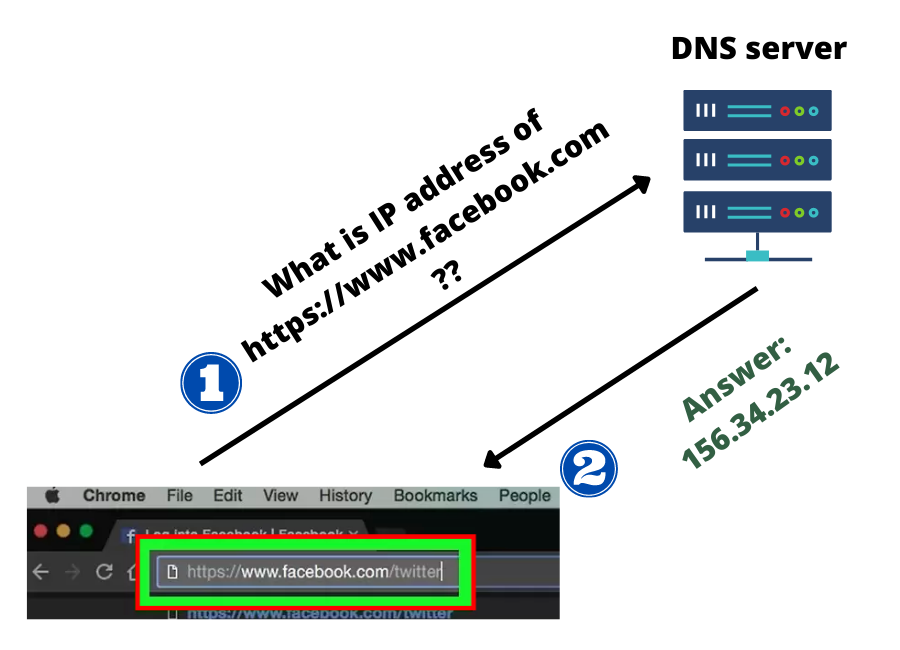
\includegraphics[scale=0.45]{content/chapter14/images/dns.png}
				\caption{DNS name resolution}
				\label{fig:severity26}
			\end{figure}			
			\item Configuration of DNS server will be covered in \textbf{Learn Linux with Lavatech Technology Part-2} book.
		\end{itemize}
	\end{itemize}
	
 \end{flushleft}
\newpage


